\newcommand{\colontitulAutors}{edombek, astronom\_v\_cube}
\newcommand{\colontitulYear}{2022}
\newcommand{\colontitulEducationalSubject}{Специальная теория относительности}
\newcommand{\colontitulTeacher}{И.~А.~Павличенко}

\documentclass[10pt,landscape,a4paper]{article}
\usepackage[utf8]{inputenc}
\usepackage[english, russian]{babel}
\usepackage[T1,T2A]{fontenc}  
\usepackage{upgreek} % прямые греческие ради русской традиции
\usepackage{tikz}
\usetikzlibrary{shapes,positioning,arrows,fit,calc,graphs,graphs.standard}
%\usepackage[nosf]{kpfonts}
%\usepackage[t1]{sourcesanspro}
\usepackage{multicol}
\usepackage{wrapfig}
\usepackage[top=6mm,bottom=8mm,left=4mm,right=4mm]{geometry}
\usepackage[framemethod=tikz]{mdframed}
\usepackage{microtype}
\usepackage{pdfpages}
\usepackage{amsthm,amsmath,amscd}   % Математические дополнения от AMS
\usepackage{amsfonts,amssymb}       % Математические дополнения от AMS
\usepackage{mathtools}              % Добавляет окружение multlined
\usepackage{xfrac}                  % Красивые дроби
\usepackage{physics}

\usepackage{fancyhdr} % колонтитулы

%некоторые математические команды
\newcommand{\Div}{\operatorname{div}}
\newcommand{\Grad}{\operatorname{grad}}

\let\bar\overline

\definecolor{myblue}{cmyk}{1,.72,0,.38}

\def\firstcircle{(0,0) circle (1.5cm)}
\def\secondcircle{(0:2cm) circle (1.5cm)}

\colorlet{circle edge}{myblue}
\colorlet{circle area}{myblue!5}

\tikzset{filled/.style={fill=circle area, draw=circle edge, thick},
	outline/.style={draw=circle edge, thick}}

\pgfdeclarelayer{background}
\pgfsetlayers{background,main}

%\everymath\expandafter{\the\everymath \color{myblue}}
\everydisplay\expandafter{\the\everydisplay \color{myblue}}

\renewcommand{\baselinestretch}{.8}
\pagestyle{empty}

\global\mdfdefinestyle{header}{%
	linecolor=gray,linewidth=1pt,%
	leftmargin=0mm,rightmargin=0mm,skipbelow=0mm,skipabove=0mm,
}

\makeatletter % Author: ttps://tex.stackexchange.com/questions/218587/how-to-set-one-header-for-each-page-using-multicols
\renewcommand{\section}{\@startsection{section}{1}{0mm}%
	{.2ex}%
	{.2ex}%x
	{\color{myblue}\sffamily\small\bfseries}}
\renewcommand{\subsection}{\@startsection{subsection}{1}{0mm}%
	{.2ex}%
	{.2ex}%x
	{\sffamily\bfseries}}

\makeatother
\setlength{\parindent}{0pt}

%колонтитулы
\pagestyle{fancy}
\fancyhf{}
\setlength{\headheight}{40pt}
\setlength{\headsep}{4pt}
\renewcommand{\headrulewidth}{1pt}
\fancyhead[L]{\textcopyright~\colontitulAutors}
\fancyhead[C]{Программа минимум по курсу <<\colontitulEducationalSubject>> \colontitulYear г}
\fancyhead[R]{Преподаватель:~\colontitulTeacher}

\begin{document}
	\small
	\begin{multicols*}{2}
		\section{Постулаты Эйнштейна}
		
		\subsection{Постулат относительности}
		
		\textbf{Законы природы одинаковы во всех ИСО.} Другими словами, законы природы \textbf{ковариантны} по отношению к преобразованиям координат и времени от одной инерциальной СО к другой. Это значит, что уравнения, описывающие некоторый закон природы и выраженные через координаты и время различных ИСО, имеют один и тот же вид.
		
		\subsection{Постулат постоянства скорости света}
		
		\textbf{Скорость света не зависит от движения источника и равнас во всех ИСО и по всем направлениям.}
		
		\section{Каноническая форма уравнений Максвелла в вакууме: 4-потенциал и 4-плотность тока в 4-пространстве}
		
		$ \bar{x} = \left(x, y, z, ict\right) $ \\
		$ \Box \bar{A} = -\dfrac{4\pi}{c}\bar{j},~ div{\bar{A}} = 0,~ div{\bar{J}} = 0~ \left(\Delta -\dfrac{1}{c^2}\dfrac{\partial^2}{\partial t^2}=\sum\limits_{s=1}^4\dfrac{\partial^2}{\partial x_s^2}=\Box\right) $  \\
		$ \bar{A} = \left(A_x, A_y, A_z, i\phi\right) \text{-четырёхпотенциал},~ \bar{J} = \left(j_x, j_y, j_z, ic\rho\right) \text{-четырёхплотность тока} $
		
		\section{Интервал между мировыми координатами двух событий в ИСО. Инвариантность интервала}
		
		Интервал является инвариантом по отношению к преобразованию Лоренца. Это значит, что два события, разделенные пространственно- подобным интервалом в одной ИСО, разделены пространственно-подобным интервалом такой же величины и в любой другой ИСО. Аналогично два события, разделённые времени-подобным интервалом в одной СО, разделены таким же времени-подобным интервалом в любой иной ИСО.
		
		\section{Преобразования Лоренца}
		
		(частный случай, движение только по $ z $) \\ 
		$ x=x',~ y=y',~ z=\dfrac{z'+vt'}{\sqrt{1-\beta^2}},~ t=\dfrac{t'+\frac{vz'}{c^2}}{\sqrt{1-\beta^2}}~\Leftrightarrow~ z'=\dfrac{z-vt}{\sqrt{1-\beta^2}},~ t'=\dfrac{t-\frac{vt}{c^2}}{\sqrt{1-\beta^2}} $
		
		\section{Световой конус и мировые линии в 4-мерном пространстве}
		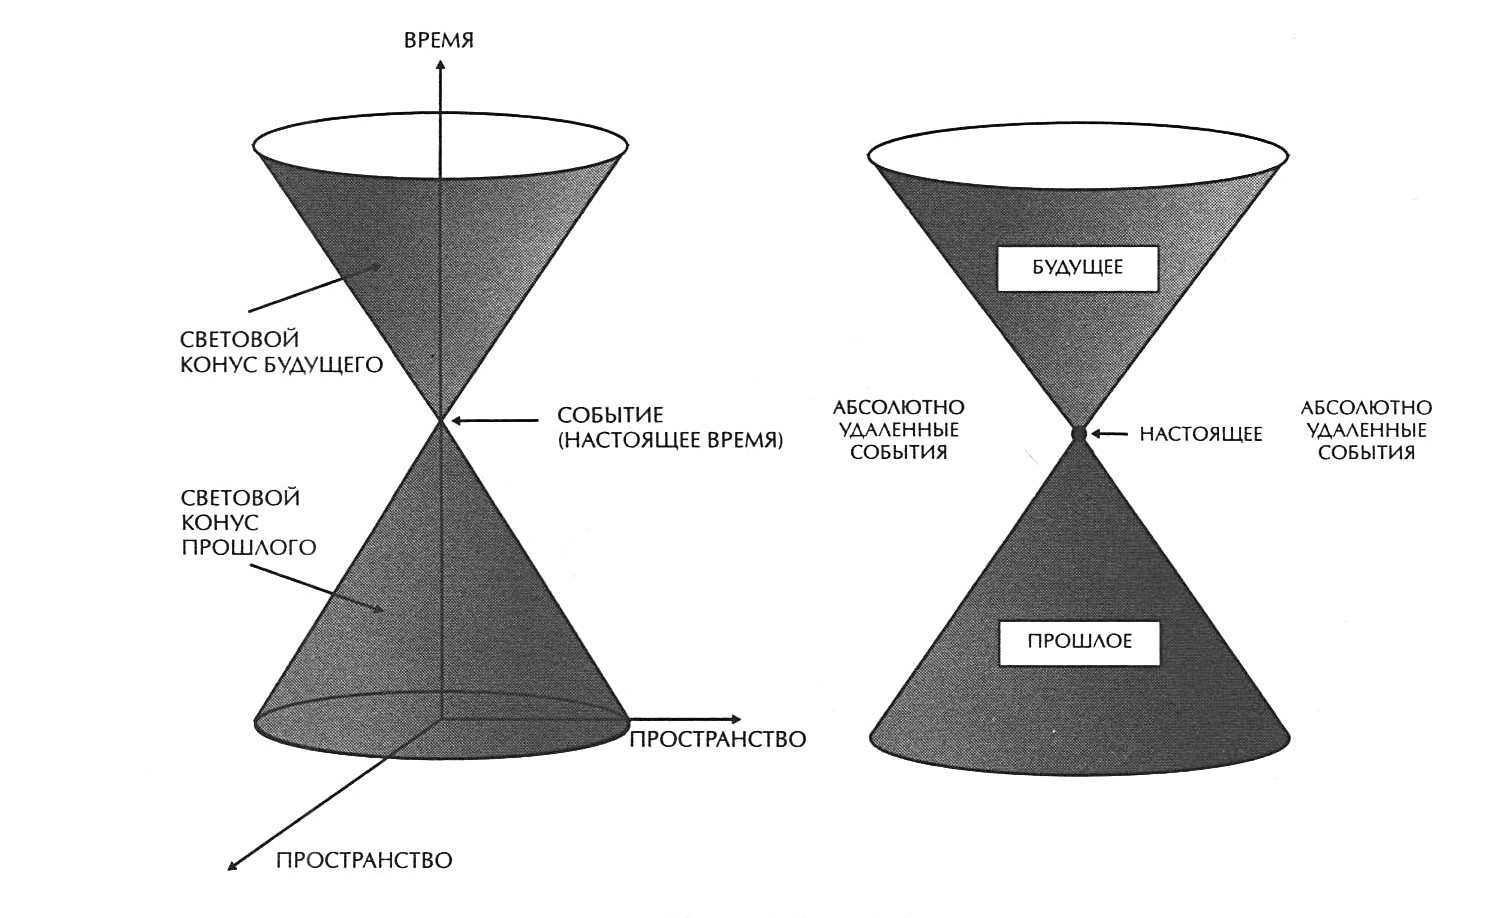
\includegraphics[width=0.6\linewidth]{sto_img/lihgt_konus}
		
		\section{Относительность одновременности двух событий}
		
		События, одновременные в ИСО К - разновременные в ИСО К'. Два одновременных события не могут быть причинно-следственно связаны.
		
		\section{Собственное время объекта}
		
		\textbf{Собственное время объекта} - время которое показывают часы двигающиеся вместе с объектом. \\
		СО  связная с часами неинерциальная. Разбиваем траекторию на маленькие кусочки где СО будет инерциальной, тогда: \\
		$ dt=\dfrac{dt'}{\sqrt{1-\beta^2}} = \dfrac{dt'}{\sqrt{1-\frac{v^2}{c^2}}} ~\Rightarrow~ dt'=dt\sqrt{1-\beta^2} ~\Rightarrow~ t_2'-t_1' = \int\limits_{t_1}^{t^2}\sqrt{1-\beta^2} $ \\
		(связь собственными ($ t' $) и неподвижными ($ t  $) часами)
		
		\section{Лоренцево сокращение длины движущегося масштаба}
		
		$ z_1'= \dfrac{z_1-vt_1}{\sqrt{1-\beta^2}},~ z_2'= \dfrac{z_2-vt_2}{\sqrt{1-\beta^2}} ~ (t_1=t_2)$ - концы движутся вместе \\
		$ z_2'-z_1' = \dfrac{z_2-z_1}{\sqrt{1-\beta^2}} ~ \Rightarrow ~ L_0 = \dfrac{L}{\sqrt{1-\beta^2}}, L = L_0\sqrt{1-\beta^2} $
		
		\section{Закон сложения скоростей}
		$V_\text{отн} = \dfrac{V+V^\prime}{1+\dfrac{VV^\prime}{c^2}}$
		
		\section{Эффект Допплера}
		$\omega^\prime = \dfrac{\omega - (k_z V)}{\sqrt{1-\beta^2}}, \quad k_z^\prime = \dfrac{k_z - ((\omega V)/c^2)}{\sqrt{1-\beta^2}}$

		\section{Действие и функция Лагранжа свободной материальной частицы в ИСО}
		$L = -m_0c^2 \sqrt{1-\beta^2}, \quad S_d = \int_{t_1}^{t_2} L(U^2) \,dt, \quad L = L(\vec{U}^2) = T-U $ - функция Лагранжа\\
		$U$ не зависит от $\vec{r}$, так как пространство однородное, $U$ и $T$ не зависят от времени, так как оно однородно, $L$ и $T$ зависят только от $\vec{V}$, $L$ зависит только от направления $\vec{V}$\\
		Действие $S_d$ - инвариант, так как во всех СО все явления должны происходить одинаково, и не существует какой-либо выделенной СО
		
		\section{Импульс и энергия свободной материальной частицы}
		$\vec{P} = \bigtriangledown_{\vec{v}}L = \dfrac{m_0\vec{V}}{\sqrt{1-\beta^2}}, \quad L = T-U$\\
		$W = (\vec{P}\vec{V})-L = \dfrac{m_0c^2}{\sqrt{1-\beta^2}}$\\
		При $V = 0$ получим конечную величину $W_0 = m_0c^2$ - энергия покоя
		
		\section{Уравнение движения релятивистской частицы в 3-мерном пространстве}
		$\dfrac{m_0}{\sqrt{1-\beta^2}}\dfrac{d\vec{V}}{dt} + \dfrac{m_0 \vec{V}}{c^2(\sqrt{1-\beta^2})^3}\vec{V} \dfrac{d\vec{V}}{dt} = \vec{f}$\\
		Первое слагаемое - перпендикулярная к скорости компонента силы, второе - продольная
		
		\section{4-скорость и 4-импульс свободной материальной частицы}
		4-х скорость - закон преобразования скорости при повороте системы координат:\\
		$\bar{U} = (\dfrac{\vec V}{\sqrt{1-\beta^2}}, \dfrac{ic}{\sqrt{1-\beta^2}}) = \dfrac{\bar{R}}{d\tau}, \quad \vec{U} \neq 0,\quad (\bar{U}\bar{U}) = -c^2$\\
		4-х импульс - параллелен 4-х скорости: $\bar{P} = m_0\bar{U} = (\dfrac{m_0\vec{V}}{\sqrt{1-\beta^2}}, i\dfrac{m_0c}{\sqrt{1-\beta^2}})$\\
		$\tau$ - собственное время объекта
		
		\section{Ковариантная форма уравнения движения частицы в ИСО и 4-сила Минковского}
		$\dfrac{d\bar{P}}{d\tau} = \bar{F},\quad \bar{F} = (\dfrac{\vec{f}}{\sqrt{1-\beta^2}}, \dfrac{i}{c}\dfrac{(\vec{f}\vec{V})}{\sqrt{1-\beta^2}})$
		
		\section{Тензор электромагнитного поля и ковариантная форма уравнений электродинамики в вакууме}
		$F = \begin{vmatrix}
			0& B_{z}& -B_{y}& -iE_x\\
			-B_{z}& 0& B_{x}& -iE_y\\
			B_{y}& -B_{x}& 0& -iE_z\\
			iE_x& iE_y& iE_z& 0 \\
		\end{vmatrix}$ - тензор электромагнитного поля;~~
		$a_{kl} = \begin{vmatrix}
			1& 0& 0& 0\\
			0& 1& 0& 0\\
			0& 0& \gamma & i\beta \gamma \\
			0& 0& -i\beta \gamma& \gamma  \\
		\end{vmatrix}$\\
		$\sum_{k}^{} \dfrac{\partial F_{ik}}{\partial x_k} = \dfrac{4\pi}{c}j_i$, \quad $\dfrac{\partial F_{ik}}{\partial x_l} + \dfrac{\partial F_{li}}{\partial x_k} + \dfrac{\partial F_{kl}}{\partial x_i} = 0$ - уравнения Максвелла в ковариантной форме\\
		$F_{ik} = a_{kl} a_{im} F_{lm}$
		
		\section{Форма и содержание закона преобразования полей}
		${\vec{B}_{\parallel}}^\prime = \vec{B}_{\parallel}, \quad {\vec{B}_{\perp}}^\prime = \dfrac{{B}_{\perp} - \dfrac{\left[\vec{V}\times \vec{E}\right]}{c}}{\sqrt{1-\beta^2}}$\\
		${\vec{E}_{\parallel}}^\prime = \vec{E}_{\parallel}, \quad {\vec{E}_{\perp}}^\prime = \dfrac{{\vec{E}}_{\perp} + \dfrac{1}{c}\left[\vec{V}\times \vec{B}\right]}{\sqrt{1-\beta^2}}$
		
		\section{Инварианты тензора электромагнитного поля}
		1. $F_{ij}\cdot F_{ij} = inv \Rightarrow \vec{E}^2-\vec{B}^2 = inv$\\
		2. $F_{ij}\cdot \tilde{F_{ij}}  = inv \Rightarrow (\vec{E}\cdot \vec{B}) = inv$\\
		Следствия:\\
		$\divideontimes$ Если в некоторой СО $E$>$B$ - выполняется в любой СО\\
		$\divideontimes$ Если в некоторой СО $\vec{E}\perp \vec{B}$ - выполняется в любой СО\\
		$\divideontimes$ Если в некоторой СО $(\vec{E}\cdot \vec{B})$ - то существует СО, где или $\vec{E} = 0$, или $\vec{B} = 0$\\
		$\divideontimes$ Если в некоторой СО или $\vec{E} = 0$, или $\vec{B} = 0$ - то в любой другой $\vec{E}\perp \vec{B}$
		
		\section{4-вектор плотности силы Лоренца и его связь с тензором электромагнитного поля}
		$\vec{f} = \rho (\vec{E} + \dfrac{1}{c}\left[\vec{V}\vec{B}\right])$ - плотность силы Лоренца\\
		$\bar{f} = (\vec{f}, \dfrac{i}{c}(\vec{f}\vec{V}))$ - 4-х вектор плотности силы Лоренца\\
		$\bar{f} = \dfrac{1}{c}(\hat{F}\bar{j}), \quad \hat{F}$ - тензор э/м поля,\quad $f_i = \dfrac{1}{c}\sum_{k}^{}F_{ik}j_k, \quad \vec{j} = \rho \vec{V}$
		
		\section{4-вектор плотности силы Лоренца и его связь с электромагнитным тензором энергии-импульса}
		$T = \begin{vmatrix}
			T_{11}& T_{12}& T_{13}& -\frac{iS_x}{c}\\
			T_{21}& T_{22}& T_{23}& -\frac{iS_y}{c}\\
			T_{31}& T_{32}& T_{33}& -\frac{iS_z}{c}\\
			-\frac{iS_x}{c}& -\frac{iS_y}{c}& -\frac{iS_z}{c}& \omega \\
		\end{vmatrix}$ - э/м тензор энергии-импульса\\
		$S = \dfrac{1}{4\pi}\left[\vec{E}\times \vec{B}\right]$ - вектор Пойтнинга, \quad $\omega = \dfrac{1}{8\pi}(\vec{E}^2 + \vec{B}^2)$ - плотность энергии\\
		$T_{\alpha \beta} = \dfrac{1}{4\pi}(E_\alpha E_\beta + B_\alpha B_\beta - \frac{1}{2}\delta_{\alpha \beta}(\vec{E}^2 + \vec{B}^2))$\\
		$\bar{f} = (\vec{f}, \dfrac{i}{c}(\vec{f}, \vec{V}))$ - 4-вектор плотности силы Лоренца\\
		$f_i = \sum_{k}^{} \dfrac{\partial T_{ik}}{\partial x_k}$ - связь с тензором

		\section{Закон сохранения энергии в электродинамике}
		$\dfrac{\partial \omega}{\partial t} + div \vec{S} + (\vec{j}E) = 0, \quad (\vec{j}E)$ - джоулевы потери\\
		$\vec{S} = \dfrac{1}{4\pi}\left[\vec{E}\times \vec{B}\right]$ - вектор Пойтнинга,\quad $\omega = \dfrac{1}{8\pi}(\vec{E}^2 + \vec{B}^2)$ - плотность энергии
		
		\section{Закон сохранения импульса в электродинамике}
		
		\section{Действие и функция Лагранжа заряженной частицы в заданном электромагнитном поле}
		$dS_g = -mc^2\sqrt{1-\beta^2} dt + (q/c(\vec{A}\vec{V}) - q\varphi)dt$ - действие заряженной частицы\\
		$L = -mc^2\sqrt{1-\beta^2} + q/c(\vec{A}\vec{V}) - q\varphi$ - функция Лагранжа
		
		\section{Импульс заряженной частицы в заданном электромагнитном поле}
		$\vec{\mathsf{P}_q} = (\dfrac{\partial L}{\partial V_q}) = \dfrac{m_0\vec{V}}{\sqrt{1-\beta^2}} + \dfrac{q}{c}\vec{A}$ - обобщенный импульс\\
		$\vec{\mathsf{P}} = \vec{P} + \dfrac{q}{c}\vec{A}$, \quad $\vec{P}$ - обычный импульс
		
		\section{Энергия заряженной частицы в заданном электромагнитном поле}
		$W_q = \dfrac{mc^2}{\sqrt{1-\beta^2}} + q\varphi = W + q\varphi$
		
		\section{Уравнение движения заряженной частицы в заданном электромагнитном поле}
		$\dfrac{d\vec{P}}{dt} = -\dfrac{q}{c}\dfrac{\partial \vec{A}}{\partial t} - q\nabla \varphi + \dfrac{q}{c}\left[\vec{V}\times rot\vec{A}\right], \quad \dfrac{d\vec{P}}{dt} = qE + \dfrac{q}{c}\left[\vec{V}\times \vec{B}\right] $
		
		\section{Поле равномерно движущегося заряда}
		
		\section{Потенциалы Льенара-Вихерта неравномерно движущегося заряда. Выражение для поля излучения}
		
		\section{Излучение неравномерно движущегося на малой скорости заряда (формула Лармора)}
		
		\section{Тормозное излучение заряда}
		
		\section{Синхротронное (магнитотормозное) излучение заряда}
		
		\section{Излучение Вавилова-Черенкова}
		
		\section{Гипотезы теории электромагнитной массы и радиус электрона}
		
		\section{Сила реакции излучения и уравнение Абрагама-Лоренца}
		
	\end{multicols*}
\end{document}
